\chapter{Marching cubes}
MC is a sequential traversal technique that was described by Lorensen and Cline in 1987 \cite{LorensenCline}. MC is a popular but not the oldest method for isosurface extraction. For example, Wyvill et. al. \cite{WyvillEtAl} In 1986, a radio propagation method was proposed. This method is similar to the MC method and is sometimes called the MC approach. MC and Wyvill et al. The methods differ in several ways. For example, they use different skipping orders. The iso-surfaces they extract are also different. Because of the differences and because most of the teams that described the use of the "MC" method used the Lorensen-Cline approach, we restrict the notation of MC to the Lorensen-Cline approach.
To understand how the MC algorithm works, let's take a 2D case and what might be called the "Marching Squares" algorithm.

\begin{figure}[!h]
	\caption{2D example of marching cube algorithm}
	\label{fig:MC}
	\begin{minipage}{.25\textwidth}
		\begin{subfigure}{\textwidth}
			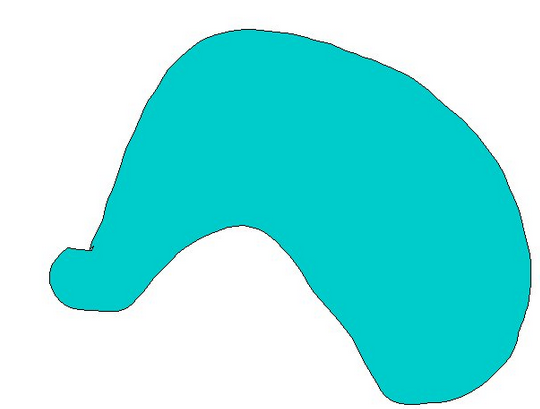
\includegraphics[width=\textwidth]{figures/MC_img.png}
			\subcaption{Reference surface}
		\end{subfigure}
		\begin{subfigure}{\textwidth}
			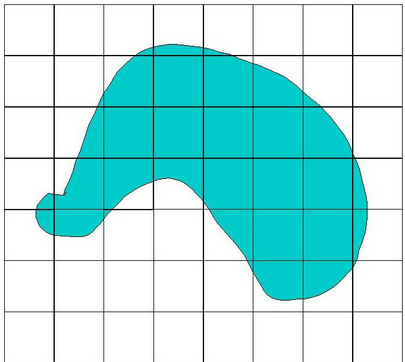
\includegraphics[width=\textwidth]{figures/MC_grid.png}
			\subcaption{Grid on top of ref surface}
		\end{subfigure}
	\end{minipage}
	\hfill
	\begin{minipage}{.25\textwidth}
		\begin{subfigure}{\textwidth}
			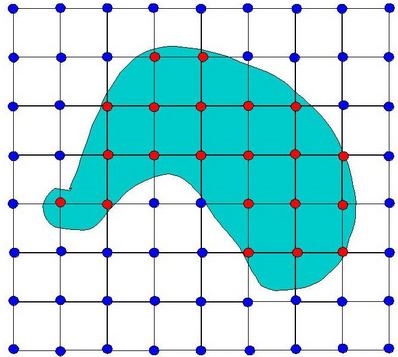
\includegraphics[width=\textwidth]{figures/MC_grid_pts.png}
			\subcaption{Identified points inside the surface}
		\end{subfigure}
		\begin{subfigure}{\textwidth}
			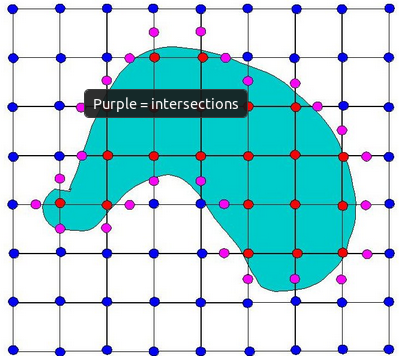
\includegraphics[width=\textwidth]{figures/MC_pts_interpolated.png}
			\subcaption{Interpolation of inside/outside points}
		\end{subfigure}
	\end{minipage}
	\hfill
	\begin{minipage}{.45\textwidth}
		\begin{subfigure}{\textwidth}
			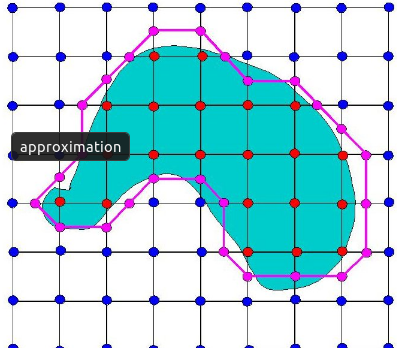
\includegraphics[width=\textwidth]{figures/MC_surface.png}
			\subcaption{2D surface reconstruction}
		\end{subfigure}
	\end{minipage}
\end{figure}
On Fig. (\ref{fig:MC}.a) reference surface is represented. Reference surface could be defined as analytical function or scalar field, which can be used later to identify, if some point in space is inside or outside the surface. In 2D case instead cubes we use squares. For each point of the grid in (\ref{fig:MC}.b) we check, if points of the square are inside or outside the surface. In (\ref{fig:MC}.c) all inside points are marked with red color, and outside points are blue. Then between inside and outside neighbouring points linear interpolation is performed to identify on-surface points (\ref{fig:MC}.d). Finally all interpolated points form a reconstructed surface as shown on Fig. (\ref{fig:MC}.e).
\paragraph{3D case.}
The same idea is used for reconstruction of 3D surface. Given scalar field function $\phi(x)$ which defines if point in space is inside or outside the surface. Generally, the high-level idea of 3D surface reconstruction can be described in the following steps:
\begin{enumerate}
	\item Determine sufficiently large bounding box of the surface.
	\item Place a uniform voxel grid in the bounding box.
	\item Compute $\phi(x)$ for all vertices in the grid. Mark vertices for which $\phi(x) \epsilon 0$.
	\item For a given edge with vertices a and b, the surface intersects the edge if $sign(\phi(a)) \neq sign(\phi(b))$. Use linear interpolation to find the intersection point along the edges. The resulting set of points are the nodes of the final triangular mesh.
	\item For each cell, determine its configuration regarding in/out vertices and query the marching cubes look up table to obtain the triangles that represent the intersection between the zero level set and the cell. Add the triangles to the final triangular mesh.
\end{enumerate}
Totally there could be 256($2^8$) cases of in/out edge displacement of the cube. Nevertheless taking in account appropriate symmetry and rotation totally there are 15 equivalent classes (Fig. \ref{fig:MC_classes}). 
\begin{figure}[h!]
	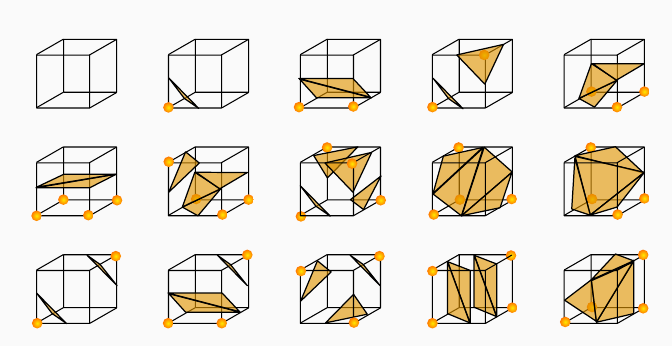
\includegraphics[width=\textwidth]{figures/MC_classes.png}
	\caption{3D marching cubes classes}
	\label{fig:MC_classes}
\end{figure}
For each class there are defined a list of points, which form a triangle mesh, thus after identifying in/out points query can be made, to get part of the triangle mesh for reconstruction of the surface. This approach is used to generate a final mesh given a computed SDF in the implemented research framework.
\paragraph{MC extensions.}
The extended algorithms was developed for handling of advanced data types, for improving computational effort of the MC algorithm or extensions that use parallel and distributing processing.

Weber et al. \cite{WeberEtAl} have extended the MC to rectilinear grid data that has a hierarchy of resolutions in certain regions. Their approach first extracts the iso-surface (using MC) separately in each sub-grid. It then forms irregularly shaped cells that are gluing together  the sub-grids.

One popularway  to  hasten  MC  has  been  to  avoid  unnecessaryoperations on the non-active (empty) cells, since 30–70\%of the processing time involves those cells \cite{Wilhelms1990}. Although some processing involving empty cells is probably inevitable, since generating a correct isosurface requires each cell to be visited at least once to learn if the cell is active, avoiding unnecessary operations on non-active cells is an effective way to accelerate the MC.

One popular method to avoid MC computations on inactive cells is to encode non-active regions in an octree \cite{WilhelmsGelder}. The octree root node refers to the entire volume. Each child node refers to an (approximately) equal-sized sub-volume of the volume described by its parent. To aid in avoiding empty cells during iso-surface construction, each octree node also stores the extremes of the region described by the node. Building the octree (i.e.,preprocessing) requires visiting each cell once and requires $O(n\cdot log(n))$ operations. However, each subsequent iso-surface extraction utilizes the octree to only visit the cells of nodes whose interval includes the 0-level. The time complexity of traversal over octree is $O\left(p + p\cdot log\left(\dfrac{n}{p}\right)\right)$, where p is a number of active cells and n is a total number of cells. Of course the naive MC traversal takes $O(n)$ operations. There are a lot of other useful method improvements described in \cite{MCSurvey}.